% Created 2021-12-10 Fri 16:21
% Intended LaTeX compiler: pdflatex
\documentclass[11pt]{article}
\usepackage[utf8]{inputenc}
\usepackage[T1]{fontenc}
\usepackage{graphicx}
\usepackage{grffile}
\usepackage{longtable}
\usepackage{wrapfig}
\usepackage{rotating}
\usepackage[normalem]{ulem}
\usepackage{amsmath}
\usepackage{textcomp}
\usepackage{amssymb}
\usepackage{capt-of}
\usepackage{hyperref}
\usepackage[margin=0.5in]{geometry}
\author{Sreejith Sreekumar}
\date{\today}
\title{Clickstream Data Processing}
\hypersetup{
 pdfauthor={Sreejith Sreekumar},
 pdftitle={Clickstream Data Processing},
 pdfkeywords={},
 pdfsubject={},
 pdfcreator={Emacs 27.2 (Org mode 9.4.4)}, 
 pdflang={English}}
\begin{document}

\maketitle
\tableofcontents





\section{Notebooks \& Code Overview}
\label{sec:orgd33134e}

\begin{itemize}
\item 1.reading.ipynb:
This notebook shows how the gzipped clickstream data is read and stored in a relational way for further processing
and analysis.

Three tables(in a mysql/mariadb database) are created during the process of parsing data.
\begin{itemize}
\item events: Every row indicates the attributes associated with a click event. A description of the event table will look as follows.

\begin{center}
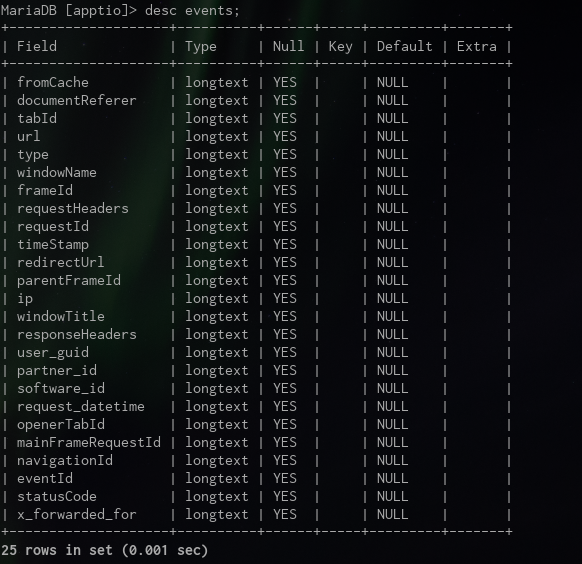
\includegraphics[height=200]{imgs/events1.png}
\end{center}

\item users: Information about the users to whom the ads were served. The same user can have same or a different ad served multiple times.

\begin{center}
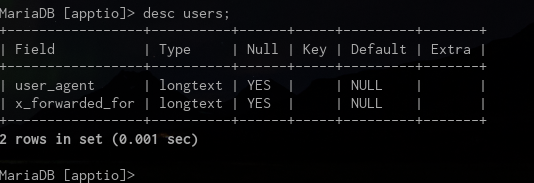
\includegraphics[height=80]{imgs/users.png}
\end{center}

\item status: Slightly less important table. Shows the description of various statuses (their codes and what they mean) during a click event.

\begin{center}
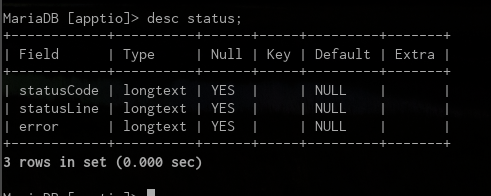
\includegraphics[height=160]{imgs/status1.png}
\end{center}
\begin{center}
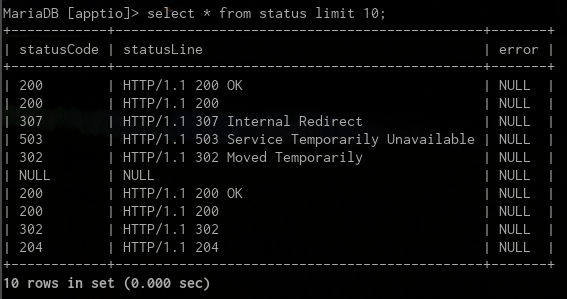
\includegraphics[height=160]{imgs/status2.png}
\end{center}
\end{itemize}

\item 2.user-cleanup.ipynb

This notebook takes the user table as input and builds a profile for every user to whom the ads were served.

\begin{center}
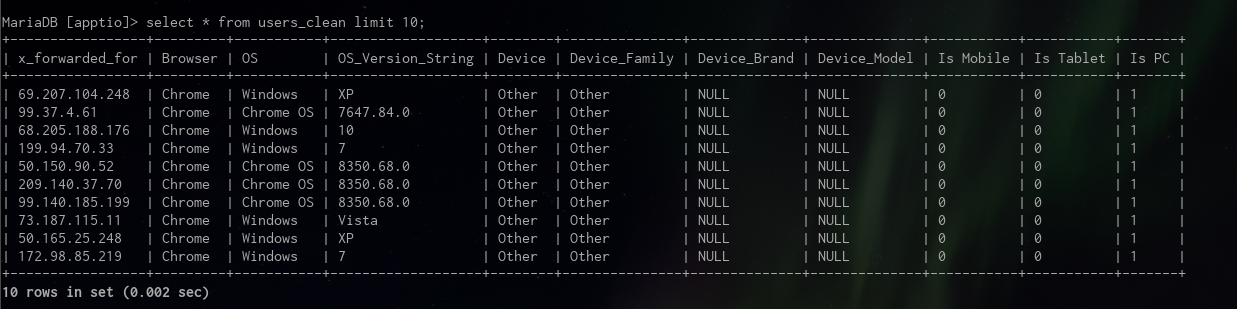
\includegraphics[width=.9\linewidth]{imgs/users-clean.png}
\end{center}

Additional attributes such as location(region, city, lat-long), ISP etc. could be extracted from the ip.
However since I was unable to find a free API, this hasn't been done.

\item 3.event-analysis.ipynb

This notebook takes the event table as input and analyses the ads served during each click event.
For instance, where was the ad referred from? Where was the landing page etc:

\begin{center}
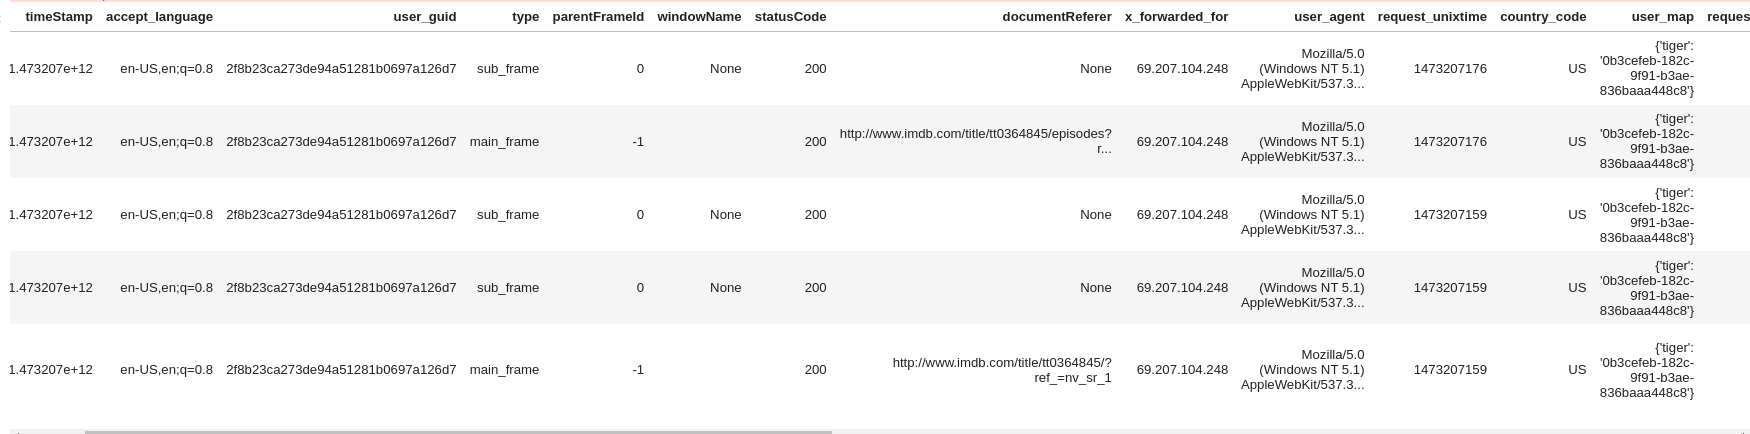
\includegraphics[height=150]{imgs/events2.png}
\end{center}

\begin{center}
Snapshot of the data kept in events table
\end{center}

\begin{center}
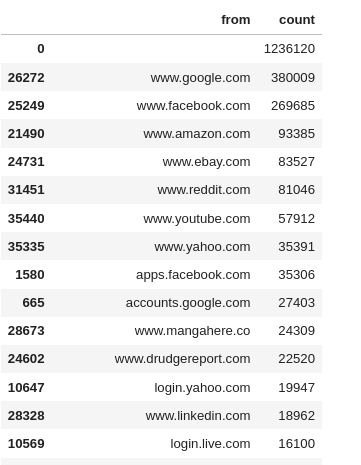
\includegraphics[height=150]{imgs/ads-referrer.png}
\end{center}

\begin{center}
Summary of click counts from a few of the top referrers
\end{center}
\end{itemize}


\section{Questions}
\label{sec:org1966948}

\subsection{How would you validate the data?}
\label{sec:org4c1dc23}
\noindent\rule{\textwidth}{0.5pt}


\begin{enumerate}
\item Make sure that the zip files are not corruped, or check why this has happened if it did. The code takes in the variable \emph{\(log\_directory\_root\)}
where a report (failed.txt) will be written if any of the gzip files fail to read.
It will also create the file (processed.txt) with a list of filenames that will be processed during the run. \\

\item \uline{Validating Headers}: Every json record inside a gzipped text has the columns '\(request\_keys\)' and '\(server\_request\_keys\)'. However not all jsons have the
same keys in the second level of hierarchy. During the first iteration of parsing, the code goes through all json instances and collects all the
available keys (headers). From the files given, 36 columns were identified. These columns are written in the file schema.txt inside the configured log directory. \\

During the second iteration of parsing the data is decoded from json and is made to a dataframe, the columns that are missing in the dataframe are found and are attached
to it with "None" as its values. This standardizes all the columns for all the data (from all the files). \\

\uline{Additional Validation}

Ideally, the validation of data could be designed like a pipeline (chain) of conditions where each dataframe goes through, for example: \\

a) Choose a subset of all the columns discovered in data \\
b) Choose a date-range for the records from each dataframe \\
c) Remove any instance where there is the error column is not null \\

These conditions have to be configurable or could be modified with very less code addition.

Note: Please see line 121 in the function \emph{\(standardize\_data\)} function in the file utils.py
\end{enumerate}

\subsection{How would you normalize the data and make it representative?}
\label{sec:orgf14d165}
\noindent\rule{\textwidth}{0.5pt}


The raw data can be split into 2 main parts. An \textbf{event} (a click) and a \textbf{user} (identified by an IP address - \(x\_forwarded\_for\)).This redundancy can be reduced by splitting the
whole data into two tables: events and users for separate analysis. \\

The attributes associated with the user comes from the \(user\_agent\) field in the request. The number of times a user has clicked an ad could also be added to this table through a groupby
of \(x\_forwarded\_for\) and \(user\_agent\). However, this needs to be done in a map reduce way since the data is too large to be held in RAM and processed.\\

The event table stores all the attributes associated with a clickevent.
This table can be used to understand the details associated with an event such as the referrer, and the landing of a click. In additional, the table provides information on when the click
happened (\(unix\_timestamp\)), when the data reached the data collection point (timeStamp), some details of the page such as frameId, tabId etc., and status of the click. 
The referrers (long urls) and the detination urls could be cleaned up to derive business insights on customer engagements. \\

The status table is a relatively small table that contains the description of every status that have appeared during a click event. \\


Note: These tables have been exported to a csv and has been shared as a link. \\
\end{document}
